% Options for packages loaded elsewhere
\PassOptionsToPackage{unicode}{hyperref}
\PassOptionsToPackage{hyphens}{url}
\PassOptionsToPackage{dvipsnames,svgnames,x11names}{xcolor}
%
\documentclass[
  letterpaper,
  DIV=11,
  numbers=noendperiod]{scrartcl}

\usepackage{amsmath,amssymb}
\usepackage{iftex}
\ifPDFTeX
  \usepackage[T1]{fontenc}
  \usepackage[utf8]{inputenc}
  \usepackage{textcomp} % provide euro and other symbols
\else % if luatex or xetex
  \usepackage{unicode-math}
  \defaultfontfeatures{Scale=MatchLowercase}
  \defaultfontfeatures[\rmfamily]{Ligatures=TeX,Scale=1}
\fi
\usepackage{lmodern}
\ifPDFTeX\else  
    % xetex/luatex font selection
\fi
% Use upquote if available, for straight quotes in verbatim environments
\IfFileExists{upquote.sty}{\usepackage{upquote}}{}
\IfFileExists{microtype.sty}{% use microtype if available
  \usepackage[]{microtype}
  \UseMicrotypeSet[protrusion]{basicmath} % disable protrusion for tt fonts
}{}
\makeatletter
\@ifundefined{KOMAClassName}{% if non-KOMA class
  \IfFileExists{parskip.sty}{%
    \usepackage{parskip}
  }{% else
    \setlength{\parindent}{0pt}
    \setlength{\parskip}{6pt plus 2pt minus 1pt}}
}{% if KOMA class
  \KOMAoptions{parskip=half}}
\makeatother
\usepackage{xcolor}
\setlength{\emergencystretch}{3em} % prevent overfull lines
\setcounter{secnumdepth}{5}
% Make \paragraph and \subparagraph free-standing
\ifx\paragraph\undefined\else
  \let\oldparagraph\paragraph
  \renewcommand{\paragraph}[1]{\oldparagraph{#1}\mbox{}}
\fi
\ifx\subparagraph\undefined\else
  \let\oldsubparagraph\subparagraph
  \renewcommand{\subparagraph}[1]{\oldsubparagraph{#1}\mbox{}}
\fi

\usepackage{color}
\usepackage{fancyvrb}
\newcommand{\VerbBar}{|}
\newcommand{\VERB}{\Verb[commandchars=\\\{\}]}
\DefineVerbatimEnvironment{Highlighting}{Verbatim}{commandchars=\\\{\}}
% Add ',fontsize=\small' for more characters per line
\usepackage{framed}
\definecolor{shadecolor}{RGB}{241,243,245}
\newenvironment{Shaded}{\begin{snugshade}}{\end{snugshade}}
\newcommand{\AlertTok}[1]{\textcolor[rgb]{0.68,0.00,0.00}{#1}}
\newcommand{\AnnotationTok}[1]{\textcolor[rgb]{0.37,0.37,0.37}{#1}}
\newcommand{\AttributeTok}[1]{\textcolor[rgb]{0.40,0.45,0.13}{#1}}
\newcommand{\BaseNTok}[1]{\textcolor[rgb]{0.68,0.00,0.00}{#1}}
\newcommand{\BuiltInTok}[1]{\textcolor[rgb]{0.00,0.23,0.31}{#1}}
\newcommand{\CharTok}[1]{\textcolor[rgb]{0.13,0.47,0.30}{#1}}
\newcommand{\CommentTok}[1]{\textcolor[rgb]{0.37,0.37,0.37}{#1}}
\newcommand{\CommentVarTok}[1]{\textcolor[rgb]{0.37,0.37,0.37}{\textit{#1}}}
\newcommand{\ConstantTok}[1]{\textcolor[rgb]{0.56,0.35,0.01}{#1}}
\newcommand{\ControlFlowTok}[1]{\textcolor[rgb]{0.00,0.23,0.31}{#1}}
\newcommand{\DataTypeTok}[1]{\textcolor[rgb]{0.68,0.00,0.00}{#1}}
\newcommand{\DecValTok}[1]{\textcolor[rgb]{0.68,0.00,0.00}{#1}}
\newcommand{\DocumentationTok}[1]{\textcolor[rgb]{0.37,0.37,0.37}{\textit{#1}}}
\newcommand{\ErrorTok}[1]{\textcolor[rgb]{0.68,0.00,0.00}{#1}}
\newcommand{\ExtensionTok}[1]{\textcolor[rgb]{0.00,0.23,0.31}{#1}}
\newcommand{\FloatTok}[1]{\textcolor[rgb]{0.68,0.00,0.00}{#1}}
\newcommand{\FunctionTok}[1]{\textcolor[rgb]{0.28,0.35,0.67}{#1}}
\newcommand{\ImportTok}[1]{\textcolor[rgb]{0.00,0.46,0.62}{#1}}
\newcommand{\InformationTok}[1]{\textcolor[rgb]{0.37,0.37,0.37}{#1}}
\newcommand{\KeywordTok}[1]{\textcolor[rgb]{0.00,0.23,0.31}{#1}}
\newcommand{\NormalTok}[1]{\textcolor[rgb]{0.00,0.23,0.31}{#1}}
\newcommand{\OperatorTok}[1]{\textcolor[rgb]{0.37,0.37,0.37}{#1}}
\newcommand{\OtherTok}[1]{\textcolor[rgb]{0.00,0.23,0.31}{#1}}
\newcommand{\PreprocessorTok}[1]{\textcolor[rgb]{0.68,0.00,0.00}{#1}}
\newcommand{\RegionMarkerTok}[1]{\textcolor[rgb]{0.00,0.23,0.31}{#1}}
\newcommand{\SpecialCharTok}[1]{\textcolor[rgb]{0.37,0.37,0.37}{#1}}
\newcommand{\SpecialStringTok}[1]{\textcolor[rgb]{0.13,0.47,0.30}{#1}}
\newcommand{\StringTok}[1]{\textcolor[rgb]{0.13,0.47,0.30}{#1}}
\newcommand{\VariableTok}[1]{\textcolor[rgb]{0.07,0.07,0.07}{#1}}
\newcommand{\VerbatimStringTok}[1]{\textcolor[rgb]{0.13,0.47,0.30}{#1}}
\newcommand{\WarningTok}[1]{\textcolor[rgb]{0.37,0.37,0.37}{\textit{#1}}}

\providecommand{\tightlist}{%
  \setlength{\itemsep}{0pt}\setlength{\parskip}{0pt}}\usepackage{longtable,booktabs,array}
\usepackage{calc} % for calculating minipage widths
% Correct order of tables after \paragraph or \subparagraph
\usepackage{etoolbox}
\makeatletter
\patchcmd\longtable{\par}{\if@noskipsec\mbox{}\fi\par}{}{}
\makeatother
% Allow footnotes in longtable head/foot
\IfFileExists{footnotehyper.sty}{\usepackage{footnotehyper}}{\usepackage{footnote}}
\makesavenoteenv{longtable}
\usepackage{graphicx}
\makeatletter
\def\maxwidth{\ifdim\Gin@nat@width>\linewidth\linewidth\else\Gin@nat@width\fi}
\def\maxheight{\ifdim\Gin@nat@height>\textheight\textheight\else\Gin@nat@height\fi}
\makeatother
% Scale images if necessary, so that they will not overflow the page
% margins by default, and it is still possible to overwrite the defaults
% using explicit options in \includegraphics[width, height, ...]{}
\setkeys{Gin}{width=\maxwidth,height=\maxheight,keepaspectratio}
% Set default figure placement to htbp
\makeatletter
\def\fps@figure{htbp}
\makeatother

% load packages
\usepackage{geometry}
\usepackage{xcolor}
\usepackage{eso-pic}
\usepackage{fancyhdr}
\usepackage{sectsty}
\usepackage{fontspec}
\usepackage{titlesec}

%% Set page size with a wider right margin
\geometry{a4paper, total={170mm,257mm}, left=20mm, top=20mm, bottom=20mm, right=50mm}

%% Let's define some colours
\definecolor{uniblue}{HTML}{003865}
\definecolor{burgundy}{HTML}{7D2239}
\definecolor{cobalt}{HTML}{005C8A}
\definecolor{lavender}{HTML}{5B4D94}
\definecolor{leaf}{HTML}{006630}
\definecolor{moss}{HTML}{385A4F}
\definecolor{pillarbox}{HTML}{B30C00}
\definecolor{rust}{HTML}{9A3A06}
\definecolor{sandstone}{HTML}{52473B}
\definecolor{skyblue}{HTML}{005398}
\definecolor{slate}{HTML}{4F5961}
\definecolor{thistle}{HTML}{951272}

%\definecolor{light}{HTML}{E6E6FA} % original from template - redefined below as uni blue at 10 percent:
\colorlet{light}{uniblue!10}
%\definecolor{highlight}{HTML}{800080} % original from template - redefined below as uni's skyblue:
\colorlet{highlight}{skyblue}
%\definecolor{dark}{HTML}{330033} % original from template - redefined below as uni blue at 100 percent:
\colorlet{dark}{uniblue}

%% Let's add the border on the right hand side 
\AddToShipoutPicture{% 
    \AtPageLowerLeft{% 
        \put(\LenToUnit{\dimexpr\paperwidth-3cm},0){% 
            \color{light}\rule{3cm}{\LenToUnit\paperheight}%
          }%
     }%
     % logo
    \AtPageLowerLeft{% start the bar at the bottom right of the page
        \put(\LenToUnit{\dimexpr\paperwidth-2.25cm},27.2cm){% move it to the top right
            \color{light}
\includegraphics[width=2.25cm]{_extensions/nrennie/PrettyPDF/uni_logo_boxed.jpg}
          }%
     }%
}

%% Style the page number
\fancypagestyle{mystyle}{
  \fancyhf{}
  \renewcommand\headrulewidth{0pt}
  \fancyfoot[R]{\thepage}
  \fancyfootoffset{3.5cm}
}
\setlength{\footskip}{20pt}

%% style the chapter/section fonts
\chapterfont{\color{uniblue}\fontsize{20}{16.8}\selectfont}
\sectionfont{\color{uniblue}\fontsize{20}{16.8}\selectfont}
\subsectionfont{\color{skyblue}\fontsize{14}{16.8}\selectfont}
\titleformat{\subsection}
  {\color{uniblue!90}\sffamily\Large\bfseries}{\thesubsection}{1em}{}[{\titlerule[0.8pt]}]
\subsubsectionfont{\color{cobalt}}

\renewcommand\thesection{\color{slate}\arabic{section}}
  
% left align title
\makeatletter
\renewcommand{\maketitle}{\bgroup\setlength{\parindent}{0pt}
\begin{flushleft}
  {\color{uniblue}\sffamily\huge\textbf{\@title}} \vspace{0.3cm} \newline
  {\Large {\@subtitle}} \newline
  \@author
\end{flushleft}\egroup
}
\makeatother

%% Use some custom fonts
\setsansfont{Ubuntu}[
    Path=_extensions/nrennie/PrettyPDF/Ubuntu/,
    Scale=0.9,
    Extension = .ttf,
    UprightFont=*-Regular,
    BoldFont=*-Bold,
    ItalicFont=*-Italic,
    ]

\setmainfont{Ubuntu}[
    Path=_extensions/nrennie/PrettyPDF/Ubuntu/,
    Scale=0.9,
    Extension = .ttf,
    UprightFont=*-Regular,
    BoldFont=*-Bold,
    ItalicFont=*-Italic,
    ]
\KOMAoption{captions}{tableheading}
\makeatletter
\@ifpackageloaded{tcolorbox}{}{\usepackage[skins,breakable]{tcolorbox}}
\@ifpackageloaded{fontawesome5}{}{\usepackage{fontawesome5}}
\definecolor{quarto-callout-color}{HTML}{909090}
\definecolor{quarto-callout-note-color}{HTML}{0758E5}
\definecolor{quarto-callout-important-color}{HTML}{CC1914}
\definecolor{quarto-callout-warning-color}{HTML}{EB9113}
\definecolor{quarto-callout-tip-color}{HTML}{00A047}
\definecolor{quarto-callout-caution-color}{HTML}{FC5300}
\definecolor{quarto-callout-color-frame}{HTML}{acacac}
\definecolor{quarto-callout-note-color-frame}{HTML}{4582ec}
\definecolor{quarto-callout-important-color-frame}{HTML}{d9534f}
\definecolor{quarto-callout-warning-color-frame}{HTML}{f0ad4e}
\definecolor{quarto-callout-tip-color-frame}{HTML}{02b875}
\definecolor{quarto-callout-caution-color-frame}{HTML}{fd7e14}
\makeatother
\makeatletter
\@ifpackageloaded{caption}{}{\usepackage{caption}}
\AtBeginDocument{%
\ifdefined\contentsname
  \renewcommand*\contentsname{Table of contents}
\else
  \newcommand\contentsname{Table of contents}
\fi
\ifdefined\listfigurename
  \renewcommand*\listfigurename{List of Figures}
\else
  \newcommand\listfigurename{List of Figures}
\fi
\ifdefined\listtablename
  \renewcommand*\listtablename{List of Tables}
\else
  \newcommand\listtablename{List of Tables}
\fi
\ifdefined\figurename
  \renewcommand*\figurename{Figure}
\else
  \newcommand\figurename{Figure}
\fi
\ifdefined\tablename
  \renewcommand*\tablename{Table}
\else
  \newcommand\tablename{Table}
\fi
}
\@ifpackageloaded{float}{}{\usepackage{float}}
\floatstyle{ruled}
\@ifundefined{c@chapter}{\newfloat{codelisting}{h}{lop}}{\newfloat{codelisting}{h}{lop}[chapter]}
\floatname{codelisting}{Listing}
\newcommand*\listoflistings{\listof{codelisting}{List of Listings}}
\makeatother
\makeatletter
\makeatother
\makeatletter
\@ifpackageloaded{caption}{}{\usepackage{caption}}
\@ifpackageloaded{subcaption}{}{\usepackage{subcaption}}
\makeatother
\makeatletter
\@ifpackageloaded{tcolorbox}{}{\usepackage[skins,breakable]{tcolorbox}}
\makeatother
\makeatletter
\@ifundefined{shadecolor}{\definecolor{shadecolor}{rgb}{.97, .97, .97}}{}
\makeatother
\makeatletter
\@ifundefined{codebgcolor}{\definecolor{codebgcolor}{named}{light}}{}
\makeatother
\makeatletter
\ifdefined\Shaded\renewenvironment{Shaded}{\begin{tcolorbox}[colback={codebgcolor}, enhanced, sharp corners, boxrule=0pt, frame hidden, breakable]}{\end{tcolorbox}}\fi
\makeatother
\ifLuaTeX
  \usepackage{selnolig}  % disable illegal ligatures
\fi
\usepackage{bookmark}

\IfFileExists{xurl.sty}{\usepackage{xurl}}{} % add URL line breaks if available
\urlstyle{same} % disable monospaced font for URLs
\hypersetup{
  pdftitle={Extra material},
  colorlinks=true,
  linkcolor={highlight},
  filecolor={Maroon},
  citecolor={Blue},
  urlcolor={highlight},
  pdfcreator={LaTeX via pandoc}}

\title{Extra material}
\author{}
\date{}

\begin{document}
\maketitle

\pagestyle{mystyle}

\section{Ordinal logistic regression}\label{ordinal-logistic-regression}

In the car preferences example there was a natural ordering among the
response categories for the importance of power steering and air
conditioning when buying a car: ``no/little importance'', ``important'',
``very important''. This ordering can be taken into account in the model
specification. Such ordering often arises in market research, opinion
polls and questionnaires (\emph{e.g.} student feedback at the University
of Glasgow).

\subsection{Latent variable view of ordered
responses}\label{latent-variable-view-of-ordered-responses}

Sometimes an ordinal response could arise if there is a continuous
variable \(Z\), such as severity of disease, which is hard to measure.
\(Z\) is a \textbf{latent variable}, because it cannot be observed
directly. Instead, cutpoints \(C_j\) are identified so that, for
instance, patients have ``no disease'', ``mild disease'', ``moderate
disease'' or ``severe disease'' corresponding to values of \(Z\) from
low to high. \(C_1, \dots, C_{J-1}\) identify \(J\) ordered categories
with associated probabilities \(p_1,p_2,\dots, p_J\). An example of the
continuous distribution of \(Z\) with cutpoints for four categories is
shown below. Here, four discrete responses can occur depending on the
position of \(Z\) relative to the cutpoints \(C_j\).

\begin{center}
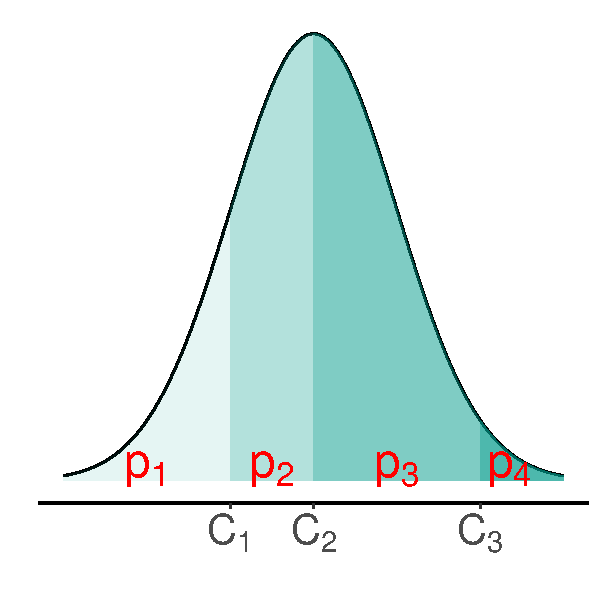
\includegraphics{about_files/figure-pdf/unnamed-chunk-1-1.pdf}
\end{center}

\subsection{Proportional odds logistic regression
model}\label{proportional-odds-logistic-regression-model}

There are several ways in which to model logits involving the
probabilities \(p_j\). The most commonly used model is the
\textbf{proportional odds logistic regression model}. If the linear
predictor \(\boldsymbol{x}^\intercal \boldsymbol{\beta}_j\) has an
intercept term \(\beta_{0j}\) which depends on category \(j\), but the
other explanatory variables do not depend on \(j\), then the model is

\[
\log \left(\frac{p_1+p_2+\dots+p_j}{p_{j+1}+\dots+p_J}\right)=\beta_{0j}+\beta_1 x_1 + \dots + \beta_{p-1}x_{p-1}. 
\]

This is called the \textbf{proportional odds model} and is based on the
assumption that the effects of the covariates \(x_1,\dots, x_{p-1}\) are
the same for all categories on the logarithmic scale, as illustrated in
the figure below.

\begin{center}
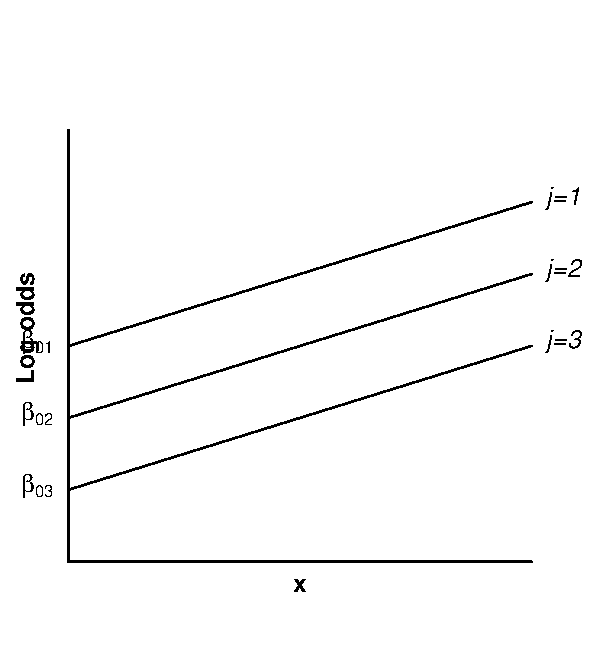
\includegraphics{about_files/figure-pdf/unnamed-chunk-2-1.pdf}
\end{center}

\begin{tcolorbox}[enhanced jigsaw, coltitle=black, opacitybacktitle=0.6, title=\textcolor{quarto-callout-note-color}{\faInfo}\hspace{0.5em}{Note}, titlerule=0mm, toprule=.15mm, bottomtitle=1mm, colback=white, colbacktitle=quarto-callout-note-color!10!white, arc=.35mm, leftrule=.75mm, breakable, bottomrule=.15mm, rightrule=.15mm, toptitle=1mm, left=2mm, opacityback=0, colframe=quarto-callout-note-color-frame]

Some alternatives to the proportional odds model for ordinal responses
are given below.

\begin{itemize}
\tightlist
\item
  Cumulative logit model
\end{itemize}

The cumulative odds for the \(j\)th category are
\[\frac{\Pr(Z\leq C_j)}{\Pr(Z>C_j)}=\frac{p_1+p_2+\dots+p_j}{p_{j+1}+\dots+p_J}\]
The cumulative logit model is
\[\log \left(\frac{p_1+p_2+\dots+p_j}{p_{j+1}+\dots+p_J}\right)=\boldsymbol{x}^\intercal \boldsymbol{\beta}_j.\]

\begin{itemize}
\tightlist
\item
  Adjacent categories logit model
\end{itemize}

If we consider ratios of probabilities, \emph{e.g.}
\(\frac{p_1}{p_2}, \frac{p_2}{p_3},\dots, \frac{p_{J-1}}{p_J}\) we can
define the adjacent category logit model as

\[
 \log \left(\frac{p_j}{p_{j+1}}\right)=\boldsymbol{x}^\intercal \boldsymbol{\beta}_j, \hspace{1cm} \text{for } j=1,\dots,J-1. 
\]

If this is simplified to

\[
\log \left(\frac{p_j}{p_{j+1}}\right)=\beta_{0j}+\beta_1 x_1 + \dots + \beta_{p-1}x_{p-1}, 
\]

the effect of each explanatory variable is assumed to be the same for
all adjacent pairs of categories.

\begin{itemize}
\tightlist
\item
  Continuation ratio logit model
\end{itemize}

Another alternative is to consider the ratios of probabilities
\(\frac{p_1}{p_2}, \frac{p_1+p_2}{p_3},\dots, \frac{p_1+\dots+p_{J-1}}{p_J}\)
or
\(\frac{p_1}{p_2+\dots+p_J}, \frac{p_2}{p_3+\dots+p_J},\dots, \frac{p_{J-1}}{p_J}\).

The equation

\[
   \log \left(\frac{p_j}{p_{j+1}+\dots+p_J}\right)=\boldsymbol{x}^\intercal \boldsymbol{\beta}_j
\]

models the odds of the response being in category \(j\),
i.e.~\(C_{j-1}<Z\leq C_j\) conditional upon \(Z>C_{j-1}\).

For instance, in the car preferences data example we could estimate the
odds of respondents regarding air conditioning and power steering as
``unimportant'' vs.~``important'' or ``very important'' using
\[\log \left(\frac{p_1}{p_2+p_3}\right).\]

Similarly, the odds of these features being ``very important'' given
that they are ``important'' or ``very important'' can be estimated by
\[\log \left(\frac{p_2}{p_3}\right).\]

\end{tcolorbox}

\section{Proportional odds logistic regression model for the car
preference
data}\label{proportional-odds-logistic-regression-model-for-the-car-preference-data}

Looking at the car preference example again, we can fit the response as
an ordinal variable using a proportional odds model of the form:

\begin{equation}\phantomsection\label{eq-polr1}{
\log \left(\frac {p_1} {p_2+p_3} \right)= \beta_{01} + \beta_{1}x_1 + \beta_{2}x_2 +\beta_{3}x_3
}\end{equation}

\begin{equation}\phantomsection\label{eq-polr2}{
\log \left(\frac {p_1+p_2} {p_3}\right) = \beta_{02} + \beta_{1}x_1 + \beta_{2}x_2 +\beta_{3}x_3 
}\end{equation}

where \(j=1\) for \texttt{no/little\ importance} (also referred to as
``unimportant''), \(j=2\) for \texttt{important} and \(j=3\) for
\texttt{very\ important}, \(x_1 =1\) for women and 0 for men,
\(x_2 = 1\) for age 24-40 years and 0 otherwise and \(x_3 = 1\) for age
\(> 40\) and 0 otherwise.

We fit this model using the \texttt{polr()} function in
\texttt{library(MASS)}, which, incidentally, uses the parameterisation

\begin{equation}\phantomsection\label{eq-polr3}{
\log \left(\frac {p_1} {p_2+p_3} \right)= \beta_{01} - \beta_{1}x_1 - \beta_{2}x_2 -\beta_{3}x_3 
}\end{equation}

\begin{equation}\phantomsection\label{eq-polr4}{
\log \left(\frac {p_1+p_2} {p_3}\right) = \beta_{02} - \beta_{1}x_1 - \beta_{2}x_2 -\beta_{3}x_3 
}\end{equation}

instead of Equation~\ref{eq-polr1} and Equation~\ref{eq-polr2}

\begin{Shaded}
\begin{Highlighting}[]
\FunctionTok{library}\NormalTok{(MASS)}
\NormalTok{m4 }\OtherTok{\textless{}{-}} \FunctionTok{polr}\NormalTok{(response }\SpecialCharTok{\textasciitilde{}}\NormalTok{ sex }\SpecialCharTok{+}\NormalTok{ age, }\AttributeTok{data=}\NormalTok{ dcars, }\AttributeTok{weight =}\NormalTok{ frequency, }\AttributeTok{Hess=}\ConstantTok{TRUE}\NormalTok{)}
\FunctionTok{summary}\NormalTok{(m4)}
\end{Highlighting}
\end{Shaded}

\begin{verbatim}
Call:
polr(formula = response ~ sex + age, data = dcars, weights = frequency, 
    Hess = TRUE)

Coefficients:
          Value Std. Error t value
sexwomen 0.5762     0.2262   2.548
age24-40 1.1471     0.2776   4.132
age> 40  2.2325     0.2915   7.659

Intercepts:
                         Value  Std. Error t value
no/little|important      0.6198 0.2168     2.8588 
important|very important 2.2312 0.2546     8.7625 

Residual Deviance: 581.2956 
AIC: 591.2956 
\end{verbatim}

The intercepts correspond to the \(j\)th category, so the log odds of
considering the features ``unimportant'' is 0.620 corresponding to a
probability of 0.65 for men age 18-23. The log odds of considering the
features ``unimportant'' or ``important'' is 2.231 corresponding to a
probability of 0.903, giving a probability of 0.253 of considering the
features ``important''. This leaves a probability of 0.097 of
considering the features ``very important'' for men age 18-23. These
probabilities are calculated using equations (Equation~\ref{eq-polr3})
and (Equation~\ref{eq-polr4}) together with \(p_1+p_2+p_3=1\). For
instance for men age 18-23 (baseline) we get
\[\hat{p}_1=\frac{\exp(\hat{\beta}_{01})}{1+\exp(\hat{\beta}_{01})}=\frac{\exp(0.6198)}{1+\exp(0.6198)}=0.650\]
and
\[\hat{p}_3=\frac{1}{1+\exp(\hat{\beta}_{02})}=\frac{1}{1+\exp(2.2312)}=0.097.\]

The likelihood ratio chi-squared statistic for the proportional odds
model is 77.25, and the AIC is 591.3, both very similar to those
obtained from the corresponding nominal logistic regression model (77.84
and 596.70 respectively). There is little difference in how well the
proportional odds and nominal logistic regression models describe the
data.

More examples and details on GLMs for nominal and ordinal data can be
found in

\begin{itemize}
\item
  Chapter 5 from
  \href{http://encore.lib.gla.ac.uk/iii/encore/record/C__Rb2939999}{\textbf{Extending
  linear models with R: generalized linear, mixed effects and
  nonparametric regression models by Julian Faraway}} and in
\item
  Chapter 6 of
  \href{http://encore.lib.gla.ac.uk/iii/encore/record/C__Rb2991222}{\textbf{Regression:
  models, methods and applications by Fahrmeir et al.}}
\end{itemize}

R examples are also available from UCLA's Institute for Digital Research
and Education:

\begin{itemize}
\item
  \href{https://stats.idre.ucla.edu/r/dae/multinomial-logistic-regression/}{Nominal
  logistic regression example}
\item
  \href{https://stats.idre.ucla.edu/r/dae/ordinal-logistic-regression/}{Ordinal
  logistic regression example}
\end{itemize}



\end{document}
